\subsection{Состояние гонки}

\begin{frame}
	\tableofcontents[currentsection,currentsubsection]
\end{frame}

\begin{frame}{Упражнение}
	\begin{itemize}
		\item Возьмите \href{https://github.com/yeputons/fall-2016-paradigms/raw/master/161019/sources/03-writeln-single.c}{код}.
		\item При желании можете скачать \href{https://github.com/yeputons/fall-2016-paradigms/raw/master/161019/sources/Makefile}{Makefile}.
		\item Убедитесь, что на экран выводится строка.
		\item Запустите второй поток, который выводит на экран другую строку.
		\item Найдите место, где первая строка сменяется второй.
		\item Удивитесь.
	\end{itemize}
	\href{https://github.com/yeputons/fall-2016-paradigms/raw/master/161019/sources/04-writeln-race.c}{Код}
\end{frame}

\begin{frame}{Объяснение}
	\begin{itemize}
		\item
			Потоки выполняют команды <<одновременно>>.
			Если есть доступ к общему ресурсу (экран), то порядок не определить.
		\item
			Поэтому символы выводятся вперемешку.
		\item
			\textit{Состояние гонки} (\textit{race condition}) "--- это когда результат работы зависит от того, в каком порядке потоки выполняли команды.
		\item
			Самая популярная ошибка у начинающих.
		\item
			Операция называется \textit{атомарной}, если она всегда выполняется <<за один такт>>,
			то есть другие потоки не видят её частично выполненной.
		\item
			\t{writeln} выше не атомарна.
	\end{itemize}
\end{frame}

\begin{frame}{Упражнение}
	\begin{enumerate}
		\item Сделайте счётчик:
			\begin{itemize}
				\item Второй поток в цикле увеличивает глобальную переменную \t{data} до $N = 5 \cdot 10^8$.
				\item Основной поток (\t{main}) выводит на экран текущее значение \t{data} в цикле $M = 1000$ раз.
				\item Отключите оптимизации компилятора (ключ \t{-O2} или схожий не нужен).
			\end{itemize}
		\item Убедитесь, что программа выводит на экране увеличивающиеся значения, а в конце "--- $N$.
		\item Поиграйте со значением $M$, чтобы убедиться, что в конце всегда выводится $N$.
		\item Сделайте так, чтобы основной поток выводил на экран только чётные значения \t{data} и увеличьте $M$.
		\item Что теперь происходит?
	\end{enumerate}
	Мой код:
	\href{https://github.com/yeputons/fall-2016-paradigms/raw/master/161019/sources/05-counter.c}{счётчик},
	\href{https://github.com/yeputons/fall-2016-paradigms/raw/master/161019/sources/06-even-counter.c}{чётный счётчик}.
\end{frame}

\begin{frame}{Объяснение}
	Возможная последовательность действий:
	\begin{itemize}
		\item Основной поток: \t{if (data \% 2 == 0)} $\to \t{true}$.
		\item Второй поток: \t{data++}.
		\item Основной поток: \t{printf}.
	\end{itemize}
	Как исправить?
	\pause
	\begin{itemize}
		\item Можно на каждой итерации записать значение \t{data} в локальную \t{data\_snapshot} (снимок) и работать с ним.
		\item Работает только если чтение одной переменной атомарно.
		\item Не работает, если у нас много переменных мы не можем сделать атомарный снимок (классическая задача).
	\end{itemize}
\end{frame}

\begin{frame}{Иллюстрация}
	\begin{center}
		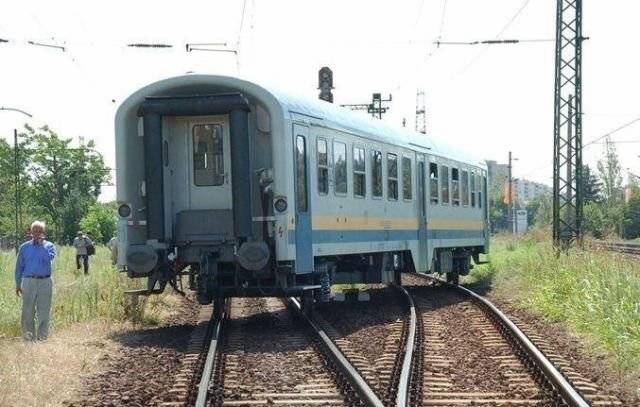
\includegraphics[scale=0.6]{race-condition.jpg}
	\end{center}
\end{frame}

\subsection{Гонка данных}
\begin{frame}{Упражнение}
	\begin{itemize}
		\item Добавьте снятие снимков в свой счётчик.
		\item Убедитесь, что все значения теперь чётные.
		\item Запустите второй поток-счётчик, который тоже увеличивает \t{data}.
		\item Что произошло?
	\end{itemize}
	Мой код:
	\href{https://github.com/yeputons/fall-2016-paradigms/raw/master/161019/sources/07-even-counter-snapshot.c}{счётчик со снимками},
	\href{https://github.com/yeputons/fall-2016-paradigms/raw/master/161019/sources/08-two-threads.c}{два счётчика}.
\end{frame}

\begin{frame}{Объяснение}
	\begin{enumerate}
		\item На уровне железа \t{data++} происходит так:
			\begin{itemize}
				\item Считай значение \t{data} из памяти.
				\item Прибавь единицу.
				\item Положи \t{data+1} на то же место в памяти.
			\end{itemize}
		\item
			Порядок операций между разными потоками произвольный.
			\begin{tabular}{cc}
				\centering
				\begin{tabular}{l|c}
					Операция & \t{data} \\ \hline
					1: \t{read} $\to 10$ & 10 \\
					1: \t{+1} $\to 11$ & 10 \\
					1: \t{write(11)} & 11 \\
					2: \t{read} $\to 11$ & 11 \\
					2: \t{+1} $\to 12$ & 11 \\
					2: \t{write(12)} & 12 \\
				\end{tabular}
				&
				\begin{tabular}{l|c}
					Операция & \t{data} \\ \hline
					1: \t{read} $\to 10$ & 10 \\
					1: \t{+1} $\to 11$ & 10 \\
					2: \t{read} $\to 10$ & 10 \\
					2: \t{+1} $\to 11$ & 10 \\
					1: \t{write(11)} & 11 \\
					2: \t{write(11)} & 11 \\
				\end{tabular}
			\end{tabular}
	\end{enumerate}
\end{frame}

\begin{frame}{А что вообще атомарно?}
	\begin{center}
		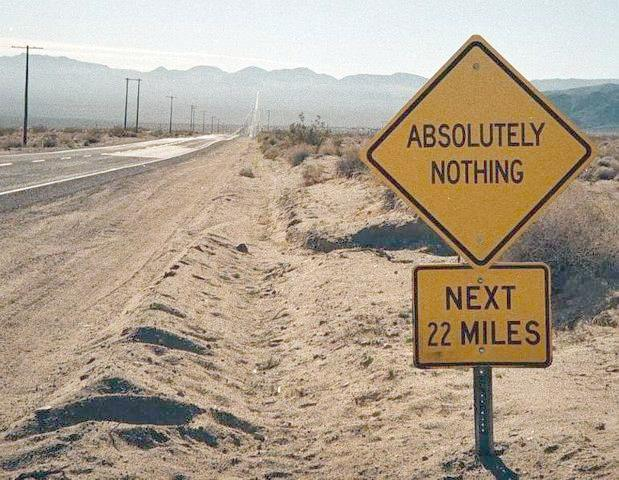
\includegraphics[scale=0.4]{absolutely-nothing.jpg}
	\end{center}
\end{frame}

\begin{frame}{Полезные советы}
	\begin{itemize}
		\item
			Что атомарно "--- очень сильно зависит от платформы, языка и ключей компиляции
			(<<модель памяти>>).
		\item Не пытайтесь угадать.
		\item Не пытайтесь самостоятельно писать код, зависящий от атомарности.
		\item В некоторых языках бывает \t{AtomicInteger} и похожие структуры.
		\item За ними тоже надо аккуратно следить, обычно не используют.
	\end{itemize}
\end{frame}
